\documentclass[a4paper, 12pt]{report}
\usepackage{graphicx}
\usepackage[swedish]{babel}
\usepackage[style=iso]{datetime2}
\usepackage{float}
\usepackage{caption}
	\captionsetup{width=.8\linewidth}
% \usepackage{subcaption,xcolor,lipsum}
\usepackage{verbatim}
% \usepackage{changepage}
\usepackage{amsmath}
\usepackage{microtype}
\usepackage{rotate}
\usepackage{siunitx}

\setlength{\parindent}{0pt}
% men däremot lite mellanrum
\setlength{\parskip}{10pt}

\usepackage{hyperref}
	\hypersetup{
		colorlinks=true,
		linkcolor=blue,
		filecolor=magenta,      
		urlcolor=cyan,
		citecolor=blue,
		pdftitle={Overleaf Example},
		pdfpagemode=FullScreen,
		}

\graphicspath{{./images/}}

\begin{document}
\begin{titlepage}
	\centering
	\includegraphics[width=0.3\textwidth]{europaskolan.png}\par\vspace{1cm}
	{\LARGE \textsc{Europaskolan Strängnäs}\par}
	\vspace{1cm}
	{\Large \textsc{Gymnasiearbete}\par}
	\vspace{1.5cm}
	{\huge\bfseries Dubbelpendeln och kaosteori \par}
	\vspace{2cm}
	{\Large\itshape Oscar Landberg \\
		KFSCI23b\par}
	\vfill
	Handledare:\par
    \vspace{-1.5mm}
	Erik Waltersson

	\vfill

	%% nedre delen av framsidan
	{\large Inlämnad: \today}
\end{titlepage}

\begin{abstract}
    Here is my Triangle. 
\end{abstract}
\chapter*{Inledning}

\section{Bakgrund}
Pendeln är något som alltid har fascinerat mänskligheten genom tiderna. Redan under det första århundradet lyckades de gamla kineserna att utveckla en seismograf med hjälp av pendeln, vars funktion funktion var att aktivera ett säkerhetssystem vid jordbävningar \cite{book:china_history}. Inte minst används också pendlar än idag; Mora-klockors tidhållning bygger på en svängande pendel, medan den klassiska metronomens tickande styrs av en inverterad variant. Det är därmed tydligt hur pendeln än idag är relevant.

På så sätt är det inte konstigt varför studiet av pendlar har länge vart en central del av fysikundervisningen, inte minst på gymnasiet. De flesta före detta (naturvetenskapliga) gymnasieelever känner säkert igen att de flesta enkla pendlarna kan beskrivas som en harmonisk svängningsrörelse, och att formeln för en pendels svängningstid är $T = 2\pi\sqrt{\frac{l}{g}}$.

Tyvärr så ingår det ingen riktig fördjupning för pendlar inom gymnasiestudierna\footnote{Det går även att argumentera för motsatsen, det kanske är bättre att lämna det åt universitetsstudenter att lära sig\dots}, och mycket av det som lärdes ut om pendlar gäller bara om startvinkeln $\theta$ är relativt liten. Det är bara när detta villkor är uppfyllt som pendlar kan beskrivas som en harmonisk svängningsrörelse, inte minst gäller detta även för svängningstidsformeln ovan.

På så vis kan en vanlig ''enkel'' pendel bli rätt så komplicerad, långt utanför gymnasiefysikens gränser. Däremot finns det många fler sätt att vidareutveckla problemet, bland annat går det att skapa en så kallad \emph{dubbelpendel} genom att koppla två enkla pendlar ihop. Det visar sig att dubbelpendeln kan väldigt enkelt visa kaotiska beteenden och bli väldigt svår att förutspå rörelsen vid, givet att startvärderna inte är helt matematiskt exakta. Därmed demonstrerar en dubbelpendel inte minst klassisk dynamik, men det är också en tydlig tillämpning på kaosteori.


%Studiet av pendlar har länge vart en central del av fysikundervisningen. De flesta gymnasieelever (som gått ett naturvetenskapligt program) känner säkert igen att de flesta vanliga pendlarna kan beskrivas som en harmonisk svängningsrörelse. Inte minst känner säkert många gymnasiefysiker igen formeln för en pendels svängningstid, $T = 2\pi\sqrt{\frac{l}{g}}$. 
%Tyvärr så ingår det ingen riktig fördjupning för pendlar inom gymnasiestudierna\footnote{Det går även att argumentera för motsatsen, det kanske är bättre att lämna det åt universitetsstudenter att lära sig\dots}, och mycket av det som lärdes ut om pendlar gäller bara om startvinkeln $\theta$ är relativt liten. Det är bara när detta villkor är uppfyllt som pendlar kan beskrivas som en harmonisk svängningsrörelse, inte minst gäller detta även för svängningstidsformeln ovan.
%På så vis kan en vanlig ''enkel'' pendel bli rätt så komplicerad, långt utanför gymnasiefysikens gränser. Däremot finns det många fler sätt att vidareutveckla problemet, bland annat går det att skapa en så kallad \emph{dubbelpendel} genom att koppla två enkla pendlar ihop. Det visar sig att dubbelpendeln kan väldigt enkelt visa kaotiska beteenden och bli väldigt svår att förutspå rörelsen vid, givet att mätdatan inte är helt perfekt. Därmed demonstrerar en dubbelpendel inte minst klassisk dynamik, men det är också en tydlig tillämpning på kaosteori. 
% Till exempel kan pendlar bara beskrivas som en harmonisk svängningsrörelse om startvinkeln $\theta$ är liten, och samma sak gäller för formeln för en pendels svängningstid.
% den välkända formeln för en matematisk pendels svängningstid $T = 2\pi\sqrt{\frac{l}{g}}$, givet att pendeln svänger runt relativt små vinklar. 
% De flesta gymnasieelever som någon gång läst fysik kommer säkert ihåg att en vanlig pendel 
% Alla som har fysik under gymnasiet känner säkert igen pendlar. De kan relativt enkelt beskrivas med 
% The study of pendulums have long been a staple of upper secondary school physics cuticulae. Not only would most upper secondary school pupil recognize that most pendulums are harmonic, but they would probably also remember the classic formula for a pendulum's period: $T = 2\pi\sqrt{\frac{l}{g}}$. 
%Pendulums are a familiar object. They are found everywhere in our daily lives; everything from the ticking of a grandfather clock, to describing the motion of a kid on a swing. The metronome, an instrument which is essential for musicians, is formed on the principle of the inverted pendulum. 
% The so-called inverted pendulum forms the fundamental basis for the operation of a metronome, which uses this principle to maintain a steady rhythm through controlled oscillations 
% They are most often found in old grandfather clocks that chime timely every hour.  
% Pendulums have long been considered a staple of upper secondary school physics curricula. 


\section{Teoretisk genomgång}
\subsection{Dubbelpendeln}
Om två vanliga enkla pendlar är sammankopplade sägs de bilda en dubbelpendel, se figur \ref{fig:double_pendulum_schematic}. Den första pendeln består av en punktformig massa $m_1$ som är kopplad till en masslös pinne med längden $l_1$, vilket sitter i en friktionslös rotationspunkt $\nu$. Den andra pendeln består också av en punktformig massa $m_2$ som är kopplad till en masslös pinne med längden $l_2$. Denna andra pendeln har sin friktionslösa rotationspunkt tillkopplad i $m_1$. Den enda kraften som verkar på respektive massa är tyngdkraften.

Låt vinklarna $\theta_1$, $\theta_2$ vara vinklarna mellan den lodräta linjen från rotationspunkten och den faktiska positionen av pendeln, se figur \ref{fig:double_pendulum_schematic}. Vinklarna $\theta_1$ och $\theta_2$ är inte begränsade mellan $-\pi \leq \theta_{1,2} \leq \pi$, dvs de kan rotera fritt hur många varv som helst runt rotationspunkterna. Detta innebär självklart att respektive pendel inte kommer påverkas av varandra, t.ex att de inte kan slå in i varandra.




% Den första pendeln består av en masslös pinne med längden $l_1$ som sitter i en friktionslös vridpunkt $\nu$. Vid änden av pinnen sitter även en punktformig massa $m_1$. Därefter kopplas en till masslös pinne med längden $l_2$ på $m_1$ så att pinnen kan rotera friktionsfritt. Dessutom finns en till punktformig massa $m_2$ tillkopplad på änden av pinnen med längden $l_2$. Eftersom pinnarna är masslösa och all friktion kan försummas, kan denna uppställning av en dubbelpendel beskrivas som en matematisk dubbelpendel. Låt vinklarna $\theta_1$, $\theta_2$ vara vinklarna normalen taket och pinnarna till för respektive enkel pendel. Den resulterande accelerationen på massorna $m_1$, $m_2$ är tyngdaccelerationen $g$.

% Eftersom pinnarna är masslösa, massorna $m_1$, $m_2$ är punktformiga och all friktion försummas, sägs dubbelpendeln vara matematisk. Därmed kommer energin i hela system bevaras. 

\begin{figure}[h]
    \centering
    %\includegraphics[scale=1]{Double-pendulum-system.png}
    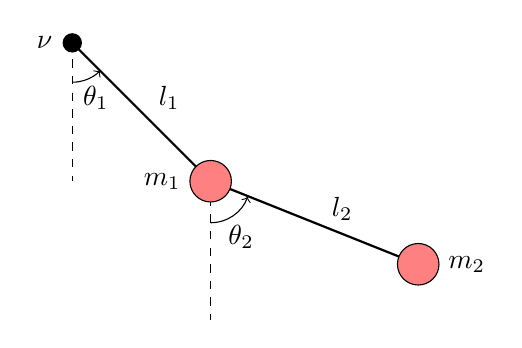
\begin{tikzpicture}

        \coordinate (O) at (0,0);

        \coordinate[yshift=-5pt,xshift=-5pt] (OL) at (O);

        \coordinate[yshift=-50pt] (OE) at (O);

        \coordinate[yshift=-50pt,xshift=50pt] (M1) at (O);

        \coordinate[yshift=-15] (MA) at (M1);

        \coordinate[yshift=-50pt] (ME) at (M1);

        \coordinate[yshift=-30pt,xshift=75pt] (M2) at (M1);

        \coordinate[yshift=-25,xshift=-25] (L) at (O);

        \draw[thick] (O) -- (M1) node[midway,xshift=10pt,yshift=5pt] {$l_1$} -- (M2) node[midway,xshift=10pt,yshift=5pt] {$l_2$};

        \draw[dashed] (O) -- (OE);

        \draw[dashed] (M1) -- (ME);


        \filldraw[color=black,fill=red!50] (M1) circle [radius=7.5pt];
        \filldraw[color=black,fill=red!50] (M2) circle [radius=7.5pt];

        \node[yshift=-20pt,xshift=8.5pt] at (O) {$\theta_1$};

        \node[yshift=-20pt,xshift=11pt] at (M1) {$\theta_2$};

        \node[xshift=-17.5pt] at (M1) {$m_1$};

        \node[xshift=17.5pt] at (M2) {$m_2$};

        %\draw[gray,ultra thick] (-3,0) -- (3,0);

        %\draw[->] (L) -- (OL);

        \node[xshift=-10pt] at (O) {$\nu$};

        % \draw[gray] (-3,0) -- (-2.5,0.35);

        % \draw[gray] (-2.5,0) -- (-2,0.35);

        % \draw[gray] (-2,0) -- (-1.5,0.35);

        % \draw[gray] (-1.5,0) -- (-1,0.35);

        % \draw[gray] (-1,0) -- (-0.5,0.35);

        % \draw[gray] (-0.5,0) -- (0,0.35);

        % \draw[gray] (0,0) -- (0.5,0.35);

        % \draw[gray] (0.5,0) -- (1,0.35);

        % \draw[gray] (1,0) -- (1.5,0.35);

        % \draw[gray] (1.5,0) -- (2,0.35);

        % \draw[gray] (2,0) -- (2.5,0.35);

        % \draw[gray] (2.5,0) -- (3,0.35);

        \fill[black] (O) circle [radius=3.5pt];

        \draw[->] (0,-0.5) arc (-90:-45:0.5);

        \draw[->] (MA) arc (-90:-20:0.5);
    \end{tikzpicture}
    \caption{Schematisk figur över en matematisk dubbelpendel.}
    \label{fig:double_pendulum_schematic}
\end{figure}

% Den enda accelerationen som verkar på massorna $m_1$, $m_2$ antas vara tyngdaccelerationen $g$. 

% vara massorna för respektive enkla pendel, och låt $l_1$, $l_2$ vara längden av respektive pendels snöre/stav. För denna rapport kommer vi bara behandla matematiska pendlar, vilket innebär att massorna $m_1$, $m_2$ antas vara punktformiga och pendels snören anses vara masslösa. 


% Även om det är rent matematiskt möjligt att härleda formlerna som beskriver en dubbelpendels rörelse med klassisk mekanik, anses det

\subsection{Lagrange-mekanik}

För att lösa mer komplexa problem, som exempelvis dubbelpendeln, är det ofta lättare att använda Lagranges ekvationer för att beskriva dess rörelse. Även om det är teoretiskt möjligt att beskriva en dubbelpendels rörelse med klassisk newtonsk mekanik, kan det fort bli mödosamt och därmed används Lagranges ekvationer istället.

En beskrivning av ett system med Lagranges ekvationer består oftast av the Lagrangian $\Lagr$ \cite{book:classical_mechanics:Morin2007}, där $T$ och $V$ är systemets kinetiska respektive lägesenergi, se ekvation (\ref{eq:Lagr}).
\begin{equation} %% todo: varför är det [2] på referensen?
    \Lagr = T - V
    \label{eq:Lagr}
\end{equation}
Sedan ger Euler-Lagrange ekvationen (\ref{eq:euler_lagrange_equation}) att den ekvation som uppfyller (\ref{eq:Lagr}) är den ekvation som beskriver systemets rörelse \cite{book:classical_mechanics:Morin2007}.
\begin{equation}
    \frac{d}{dt}\left( \frac{\partial \Lagr}{\partial \dot{q_{i}}} \right) - \frac{\partial \Lagr}{\partial q_{i}} = 0,
    \label{eq:euler_lagrange_equation}
\end{equation}
för varje $i = 1,2,3,\ldots$. Motivering och härledning av både (\ref{eq:Lagr}) och (\ref{eq:euler_lagrange_equation}) ges i appendix (TODO). %todo

\subsection{Härledning av dubbelpendels rörelseekvationer}

Härledningen utgår från figur \ref{fig:double_pendulum_schematic}, där dubbelpendeln ritats in i ett koordinatsystem där origo utgår från vridpunkten $\nu$. De punktformiga massorna $m_1$ och $m_2$ har koordinaterna $(x_1,y_1)$ respektive $(x_2,y_2)$.

Vi kan beskriva punkterna $x_1$, $x_2$, $y_1$ och $y_2$ går att beskriva genom trigonometri enligt:
\begin{align}
    x_1 & = l_1 \sin{\theta_1} \label{eq:x_1}                      \\
    y_1 & = -l_1\cos{\theta_1} \label{eq:y_1}                      \\
    x_2 & = l_1\sin{\theta_1} + l_2\sin{\theta_2} \label{eq:x_2}   \\
    y_2 & = -l_1\cos{\theta_1} - l_2\cos{\theta_2}. \label{eq:y_2}
\end{align}

Eftersom tidsderivatan av sträcka/position är hastighet, kan vi få hastigheterna $\dot{x}_1$, $\dot{y}_1$, $\dot{x}_2$ och $\dot{y}_2$ enligt:
\begin{align}
    \dot{x}_1 & = \dot{\theta}_1 l_1 \cos{\theta_1} \label{eq:x_1:dot}                   \\
    \dot{y}_1 & = \dot{\theta}_1 l_1 \sin{\theta_1} \label{eq:y_1:dot}                   \\
    \dot{x}_2 & = \dot{\theta}_1 l_1 \cos{\theta_1} + \dot{\theta}_2 l_2 \cos{\theta_2} \label{eq:x_2:dot}  \\
    \dot{y}_2 & = \dot{\theta}_1 l_1 \sin{\theta_1} + \dot{\theta}_2 l_2 \sin{\theta_2}. \label{eq:y_2:dot}
\end{align}

Vi kan därmed definiera dubbelpendelns potentiella energi $V$ som summan av den potentiella energin för respektive massa. Detta ger:
\begin{align}
    V                                              & = m_1gy_1 + m_2gy_2 \notag                                                       \\
    (\ref{eq:y_1}),\/ (\ref{eq:y_2}) \Rightarrow V & = -(m_1 + m_2)gl_1\cos{\theta_1} - m_2gl_2\cos{\theta_2}. \label{eq:V/potential_energy}
\end{align}

Vi kan också bestämma dubbelpendelns kinetiska energi $T$ enligt:
\begin{align}
    T   &= \frac{1}{2} m_1 v_{1}^{2} + \frac{1}{2}m_2v_2^2 \notag \\
        &= \frac{1}{2}m_1\left(\dot{x}_1^2 + \dot{y}_1^2\right) + \frac{1}{2}m_2\left(\dot{x}_2^2 + \dot{y}_2^2\right) \notag \\ %% TODO; motivera kanske varför v^2 = v_x^2 + v_y^2
    (\ref{eq:x_1:dot}) - (\ref{eq:y_2:dot}) \Rightarrow &= \frac{1}{2}m_1\left(\dot{\theta}_1^2 l_1^2 \cos^2{\theta_1} + \dot{\theta}_1^2 l_1^2 \sin^2{\theta_1}\right) + \frac{1}{2}m_2
    \left(
        \dot{\theta}_1^2 l_1^2 \cos^2{\theta_1}\right. \notag \\
        &\quad + 2\dot{\theta}_1\dot{\theta}_2l_1l_2\cos{\theta_1}\cos{\theta_2}
        + \dot{\theta}_2^2l_2^2\cos^2{\theta_2} \dot{\theta}_1^2l_1^2\sin^2{\theta_1} \notag \\
        &\quad + \left.2\dot{\theta}_1\dot{\theta}_2l_1l_2\sin{\theta_1}\sin{\theta_2} + \dot{\theta}_2^2l_2^2\sin^2{\theta_2}
    \right) \notag \\
    \Rightarrow &= \frac{1}{2}m_1\dot{\theta}_1^2l_1^2\left(\cos^2{\theta_1} + \sin^2{\theta_1}\right) + \frac{1}{2}m_2\left( \dot{\theta}_1^2l_1^2\left(\sin^2{\theta_1} + \cos^2{\theta_1}\right) \right. \notag \\
    &\quad + \left.\dot{\theta}_2^2l_2^2\left(\sin^2{\theta_2} + \cos^2{\theta_2}\right) 2\dot{\theta}_1\dot{\theta}_2l_1l_2\left(\cos{\theta_1}\cos{\theta_2} + \sin{\theta_1}\sin{\theta_2}\right)\right). \notag
\end{align}

Eftersom $\sin^2{\theta} + \cos^2{\theta} = 1$ och $\cos(\theta_1 - \theta_2) = \cos{\theta_1}\cos{\theta_2} + \sin{\theta_1}\sin{\theta_2}$ (trigonometriska ettan respektive subtraktionsformeln för cosinus) kan vi förenkla uttrycket till:

\begin{equation}
    T = \frac{1}{2}m_1\dot{\theta}_1^2l_1^2 + \frac{1}{2}m_2\left(\dot{\theta}_1^2l_1^2 + \dot{\theta}_2^2l_2 + 2\dot{\theta}_1\dot{\theta}_2l_1l_2\cos(\theta_1-\theta_2)\right). \label{eq:T/kinetic_energy_simplified}
\end{equation}

Nu när vi har uttryckt $V$ och $T$ som funktioner av $\theta_1$ och $\theta_2$, kan vi beräkna $\Lagr$. Enligt (\ref{eq:Lagr}), (\ref{eq:V/potential_energy}) och (\ref{eq:T/kinetic_energy_simplified}) får vi att:
\begin{align}
    \Lagr               &= T - V \notag \\
                        &= \frac{1}{2}m_1\dot{\theta}_1^2l_1^2 + \frac{1}{2}m_2\left(\dot{\theta}_1^2l_1^2 + \dot{\theta}_2^2l_2^2 + 2\dot{\theta}_1\dot{\theta}_2l_1l_2\cos(\theta_1-\theta_2)\right) \notag \\
                        &\quad - \left(-(m_1 + m_2)gl_1\cos{\theta_1} - m_2gl_2\cos{\theta_2}\right) \notag \\
    \Rightarrow \Lagr   &= \frac{1}{2}m_1\dot{\theta}_1^2l_1^2 + \frac{1}{2}m_2\left(\dot{\theta}_1^2l_1^2 + \dot                {\theta}_2^2l_2^2 + 2\dot{\theta}_1\dot{\theta}_2l_1l_2\cos(\theta_1-\theta_2)\right) \notag \\
                        &\quad + (m_1 + m_2)gl_1\cos{\theta_1} + m_2gl_2\cos{\theta_2} \label{eq:Lagr_simplified}
\end{align}

\subsubsection{Tillämpning av Euler-Lagrange ekvationen}

Vi ska nu använda ekvation (\ref{eq:Lagr_simplified}) i Euler-Lagrange ekvationen (\ref{eq:euler_lagrange_equation}) för att lösa ut ekvationen som beskriver vinklarna $\theta_1$ och $\theta_2$ i dubbelpendeln. Vi beräknar för fallet för $q_i=\theta_1$.

Deriveringsregler för att bestämma $ \frac{\partial \Lagr}{\partial \dot{\theta}_1}$ och $\frac{d}{dt}\!\left(\frac{\partial \Lagr}{\partial \dot{\theta}_1}\right)$ ger:
\begin{align}
    \frac{\partial \Lagr}{\partial \dot{\theta}_1} &= m_1l_1^2\dot{\theta}_1+ m_2l_1^2\dot{\theta}_1 + m_2l_1l_2\dot{\theta}_2\cos(\theta_1-\theta_2) \notag \\
    \Rightarrow \frac{d}{dt}\left(\frac{\partial \Lagr}{\partial \dot{\theta}_1}\right) &= m_1l_1^2\ddot{\theta}_1 + m_2l_1^2\ddot{\theta}_1 + m_2l_1l_2\ddot{\theta}_2\cos(\theta_1-\theta_2) \notag\\
    &\quad - m_2l_1l_2\dot{\theta}_2\sin(\theta_1-\theta_2)(\dot{\theta}_1-\dot{\theta}_2) \notag \\
    \Rightarrow \frac{d}{dt}\left(\frac{\partial \Lagr}{\partial \dot{\theta}_1}\right) &= \left(m_1+m_2\right)l_1^2\ddot{\theta}_1 + m_2l_1l_2\ddot{\theta}_2\cos(\theta_1-\theta_2) \notag \\
    &\quad - m_2l_1l_2\dot{\theta}_1\dot{\theta}_2\sin(\theta_1-\theta_2) + m_2l_1l_2\dot{\theta}_2^2\sin(\theta_1-\theta_2).
\end{align}

Deriveringsregler för att bestämma $\frac{\partial \Lagr}{\partial \theta_1}$ ger:
\begin{align}
    \frac{\partial \Lagr}{\partial \theta_1} &= -m_2l_1l_2\dot{\theta}_1\dot{\theta}_2\sin(\theta_1-\theta_2) - \left(m_1 + m_2\right)gl_1\sin{\theta_1}.
\end{align}

Insättning av detta i (\ref{eq:euler_lagrange_equation}) ger:
\begin{align}
    0 &=\left(m_1+m_2\right)l_1^2\ddot{\theta}_1 + m_2l_1l_2\ddot{\theta}_2\cos(\theta_1-\theta_2)
    - m_2l_1l_2\dot{\theta}_1\dot{\theta}_2\sin(\theta_1-\theta_2) \notag \\
    &\quad + m_2l_1l_2\dot{\theta}_2^2\sin(\theta_1-\theta_2) + m_2l_1l_2\dot{\theta}_1\dot{\theta}_2\sin(\theta_1-\theta_2) + \left(m_1 + m_2\right)gl_1\sin{\theta_1} \notag\\
    \Leftrightarrow 0 &= \left(m_1+m_2\right)l_1\ddot{\theta}_1 + m_2l_2\ddot{\theta}_2\cos(\theta_1-\theta_2)
    + m_2l_2\dot{\theta}_2^2\sin(\theta_1-\theta_2) \notag \\
    &\quad + \left(m_1 + m_2\right)g\sin{\theta_1}. \label{eq:theta_1_solution}
\end{align}

Därmed är (\ref{eq:theta_1_solution}) ekvationen som beskriver vinkeln $\theta_1$ i dubbelpendeln.


\end{document}